\documentclass[10pt,a4paper]{scrartcl}

\usepackage[utf8x]{inputenc}
\usepackage{ucs}
\usepackage{amsmath}
\usepackage{amsfonts}
\usepackage{amssymb}
\usepackage{graphicx}
\usepackage[british]{babel}
\usepackage{subfigure}

\setlength{\parskip}{0.5em}


\title{Sputnik}
\subtitle{Project Report HCC Project Seminar 2011}
\author{Simon Wallner\footnote{\texttt{me@simonwallner.at}}}

\begin{document}
\maketitle

\begin{abstract}
This paper evaluates \emph{Sputnik} a 3D environment with which the user can freely interact through an elastic \emph{arc of light/fishing rod} metaphor, to explore, create and interact with virtual \emph{sound objects}. These sound objects are placed in the scene and react to the user's input by sending MIDI commands to an external audio program thus creating or manipulating the sound.

\end{abstract}

\section{Reading Guide}
This report is aimed at readers with a general knowledge in computer science on the bachelor's level and above. Prior knowledge and experience with HCC and Tangible User Interfaces (TUI) is recommended, but the related work sections also includes a few introductory .. for the interested reader.

This report is accompanied by a short video, that gives a short overview and demonstrates the main interactions with Sputnik. It is advised to watch this video before reading the report. 

Also accompanying this report are the questionnaire and interview form used for the user study. They can be found in the root of this package named \texttt{questionnaire.pdf} and \texttt{interview-form.pdf}


\section{Introduction}

% setting the scene
Computer music is around us for some time now and through the use of the computer musicians have sheer endless possibilities of musical expression. With this plethora of possibilities comes the need for constraints and control to harness this expressive potential. Over the recent years many standard and non-standard interface have been developed, ranging from the ordinary button-fader-nob MIDI interface to more elaborate interfaces and systems like the \emph{reactable}\cite{Jorda2007}, \emph{mixiTUI}\cite{Pedersen2009} or commercial solutions like the \emph{Novation Launchpad}\footnote{\texttt{http://www.novationmusic.com/products/midi\_controllers/launchpad}} or \emph{Native Instruments Maschine}\footnote{\texttt{http://www.native-instruments.com/\#/en/products/producer/maschine/}} to name but a few.

With the advent of motion based controllers in consumer entertainment systems, marked by the release of the \emph{Wii}\footnote{\texttt{http://de.wikipedia.org/wiki/Wii}} console in late 2006, motion controllers became widely and cheaply available. This and their interface capabilities make them the ideal tools to explore the realm of \emph{new interfaces for musical expression}.


% problem statement
A common problem of computer music interfaces is that often the process of sound creation is not readily comprehensible. Seeing a performer on stage behind their laptop twisting knobs and adjusting faders might be ambiguous to an uninformed observer. It can be hard to relate the artist's action to the resulting sounds. This can hinder the experience and might go as far as to the point where the audience suspects that an artist just pressed play, as interviews conducted by \cite{Pedersen2009} show.

% Sputnik description
This paper introduces \emph{Sputnik}, a system that uses a \emph{Wiimote} controller to interact with a dynamic 3D scene. In the scene, a variety of sound creating objects are placed that send MIDI signals to an external audio program upon the user's interaction. 

Users can freely navigate the 3D scene and interact with it through an elastic \emph{arc of light/fishing rod} metaphor. It seems as if the \emph{arc of light} was coming out of the Wiimote and reaches into the scene, acting as an extension of the user's body into the virtual space. With this bodily extension users can \emph{grab} and \emph{drag} objects around the 3D scene.



% contribution
In this paper I evaluate the qualities of the \emph{arc or light} metaphor and how the design decisions/constraints of the system influence its expressive potential both visually and musically. This evaluation is grounded in a user study of XXX users.

Based on these findings and the theoretical framework of \cite{Ullmer2000} the similarities and differences between \emph{Sputnik} and tangible user interfaces are discussed. 


\section{Paper Outline}
The following section gives an overview over related work in the field of \emph{New Interfaces for Musical Expression} and tangible user interfaces. Section \ref{sec:results} goes into detail about Sputnik, both on a conceptual and a technical level. Section \ref{sec:evaluation} describes the performed user study and the paper is finally concluded in section \ref{sec:discussion} where the findings are discussed.


\section{Related Work}
\paragraph{Practical Work}
Only a few projects exist that go into a similar direction as Sputnik. The \emph{Virtual Xylophone}\cite{Maki-Patola2005} is a virtual reality system in which the user can place xylophone bars of different pitch in the scene and then struck them with a virtual mallet. By translating the configuration and mapping of the real instrument into the VR environment, new modes of play emerge.
\cite{Zappi2010} created a virtual controller for \emph{Ableton Live} that allows users to create simple proxy objects in a VR environment, bind them to certain controls and use them effectively as virtual sliders. \cite{Rodet2005} created a virtual environment for an exhibition setting. Users interact with the system via a 6-DOF motion tracker with tactile feedback. However, the user's actions in the system are highly constrained.

More projects can be found in the realm of Tangible User Interfaces. With \emph{mixiTUI} \cite{Pedersen2009} created a table top tangible interface for a sequencer that aimed not only to be functional but also to visually enrich the artists performance. Interviews with musicians and an extensive user study have been performed. \cite{Jorda2007} created the famous \emph{reacTable}, also a table top tangible interface that allows the creation and manipulation of music by composing various objects on its surface. 

After the release of the Wii in late 2006, the Wiimote motion controller received some attention in and outside the field of musical interfaces: 
\cite{Kiefer2008} assess the general qualities of the Wiimote as a musical controller and \cite{Miller2010} uses the Wiimote and sensor bar to create the \emph{Wiiolin}, a virtual violin that mimics the real instrument and can be played either in an upright position like a cello or horizontally like a violin. It senses the button presses and tracks the movement of the \emph{bow}, i.e. the sensor bar to create the sounds.

Not a Wiimote but still impressive, \cite{Miyama2010} uses an low resolution distance sensor array to control the many parameters of a synthesizer. A small gui application is merely used for monitoring the system's state, and sound creation is done in pd.


\paragraph{Theoretical Work}
The field of \emph{Tangible User Interfaces (TUI)} provides part of the theoretical background for this work. Work of \cite{Fitzmaurice1995} and then later \cite{Ishii1997} introduced this term and the wider concept. \cite{Shaer2009} Gives a very good overview over this field as well as the history of TUI studies. \cite{Ullmer2000} introduced \emph{MCRpd}, a formal model for describing and analysing TUIs that will be used in section \ref{}.

\cite{Sharlin2004} introduced \emph{spatial TUIs} that focuses on \emph{I/O unification} by tightly coupling the action and perception spaces and embodying a clear state representation across all sensory modalities.


Entering the musical realm \cite{Fels2011} give a good overview and general introduction into the field of \emph{NIMEs (New Interfaces for Musical Expression)}. \cite{Cook2001} shares 13 general principles for designing computer music controllers that resulted from his long lasting experience in this field. \cite{Dobrian2006} asks the question of virtuosity and expression by pointing out the elephant in the room, e.g. the lack thereof and also the lack of a comparable standard repertoire. 

In contrary to that \cite{Gurevich2007} question the hegemonic \emph{composer--interpret--listener} relation in favour of a more holistic \emph{ecological} view of musical expression. Later work by \cite{Gurevich2010} evaluated a highly constrained, prototypical one-button instrument that spurred a wide variety of play styles in test users.

Closing the loop to design and HCI, \cite{Magnusson2010} gives a good overview over the field of \emph{affordance} and elaborates on \emph{contraints} from different viewing angles and how they impact and support creativity. Finally, \cite{Wanderley2002} goes into depth over evaluating input devices for musical expression in the context of HCI. 






% ------------------------------------------------

% \cite{Magnusson2010} gives a good overview over the field of \emph{affordance} and elaborates on \emph{constraints} from different viewing anlges and how constraints impact and support creativity.

% \cite{Ullmer2000} introduces a formal model for tangible user interfaces and compares it to the prevalent MVC (Model View Controller) model. Different qualities of TUIs are stated and a few existing applications are assessed with it.

% \cite{Ishii1997} Introduced the term \emph{Tangible User Interface} (\emph{TUI}

% \cite{Kiefer2008} Assessing the potential of the wiimote as an musical interface and comparing it to a common interface. user study, only very simple mapping + perceptron shape recognition

% \cite{Wanderley2002} discusses the problems of how to assess interfaces for musical expression and searches the depths of HCI studies for a possible answer. no answer given

% \cite{Dobrian2006} tries to answer what constitutes an expressive musical interface, and how does the lack of virtuoso performers impacts the whole discussion. It highlights the role of a repertoire and the role of the performer. This is a bit contradicting to what \cite{Magnusson2010} writes.

% \cite{Cook2001} provides a few (empiric) design principles for digital musical instruments and richly illustrates them with example projects.

% \cite{Fels2011} General introduction and overview to/of the field of NIMEs given as a SIGGRAPH course. The definitive introduction to NIMEs.

% \cite{Gurevich2007} introduce an \emph{ecological} view of musical expression that goes against the conservative view of a uni-linear composer--interpret--listener relation.

% \cite{Gurevich2010} evaluate a highly constrainted one-button instrument in terms of the style and variations these constraints induce.

% \cite{Maki-Patola2005} built four virtual reality instruments for a cave like environment, one of them being a virtual mallet, where users can hit the pads with virtual mallets. This comes closest to Sputnik and also a few general thought on virtual scenes and the possible impact on the performance are given.

% \cite{Miller2010} uses the Wiimote and sensor bar to modell a virtual violin. It has no graphical UI and uses recorded sound samples.

% \cite{Miyama2010} IR distance sensor array used to control a pd patch and a simple gui application written in c.

% \cite{Pedersen2009} mixiTUI, tangible sequencer with gui, user study and interviews.

% \cite{Sharlin2004} introduces \emph{spatial TUIs} and discusses I/O unification on a few examples, coupling of action and perception space.

% \cite{Fitzmaurice1995} introduces \emph{graspable user interfaces} with Briks.

% not used
% \cite{Gamberini2011} introduces \emph{action breakdowns} for quantitative studies of user interfaces.

% \cite{Shaer2009} Give a general introduction into the field of TUIs and provide an historical overview.

% furhter research
% \cite{Godoey2006} explores the the playing of \emph{air instruments} and what is behind it. 

% \cite{Zappi2010} built a motion tracked 3d virtual environment in which users can create/bind/interact with basic virtual objects to control all aspects of a \emph{live} set. Input done via hand gestures only simple parameter mapping, virtual faders.

% \cite{Rodet2005} haptic feedback to objects in a ve, very simple interaction, no direct scene interaction.







\section{Sputnik}
\emph{Sputnik} is a \emph{New Interface for Musical Expression} that combines 3D graphics with the capabilities of the wireless \emph{Wiimote} and \emph{Nunchuck} controller. The user is presented with a colourful 3D scene that contains various interactive objects. The user can freely navigate the scene and interact with these object to create sounds.

\subsection{Setup}
The system is set up in a room with an overhead mounted video projector. The IR-sensor bar, needed for the Wiimote controller, can either be placed on the upper or lower edge of the projected image. It consists of two IR emitters that allows the IR camera in the Wiimote to track its relative orientation in space. A Wiimote and Nunchuck controller are used and only a single person at a time can use the system. Figure \ref{fig:sputnik-setup} illustrates the setup.

\begin{figure}[hbtp]
\begin{center}
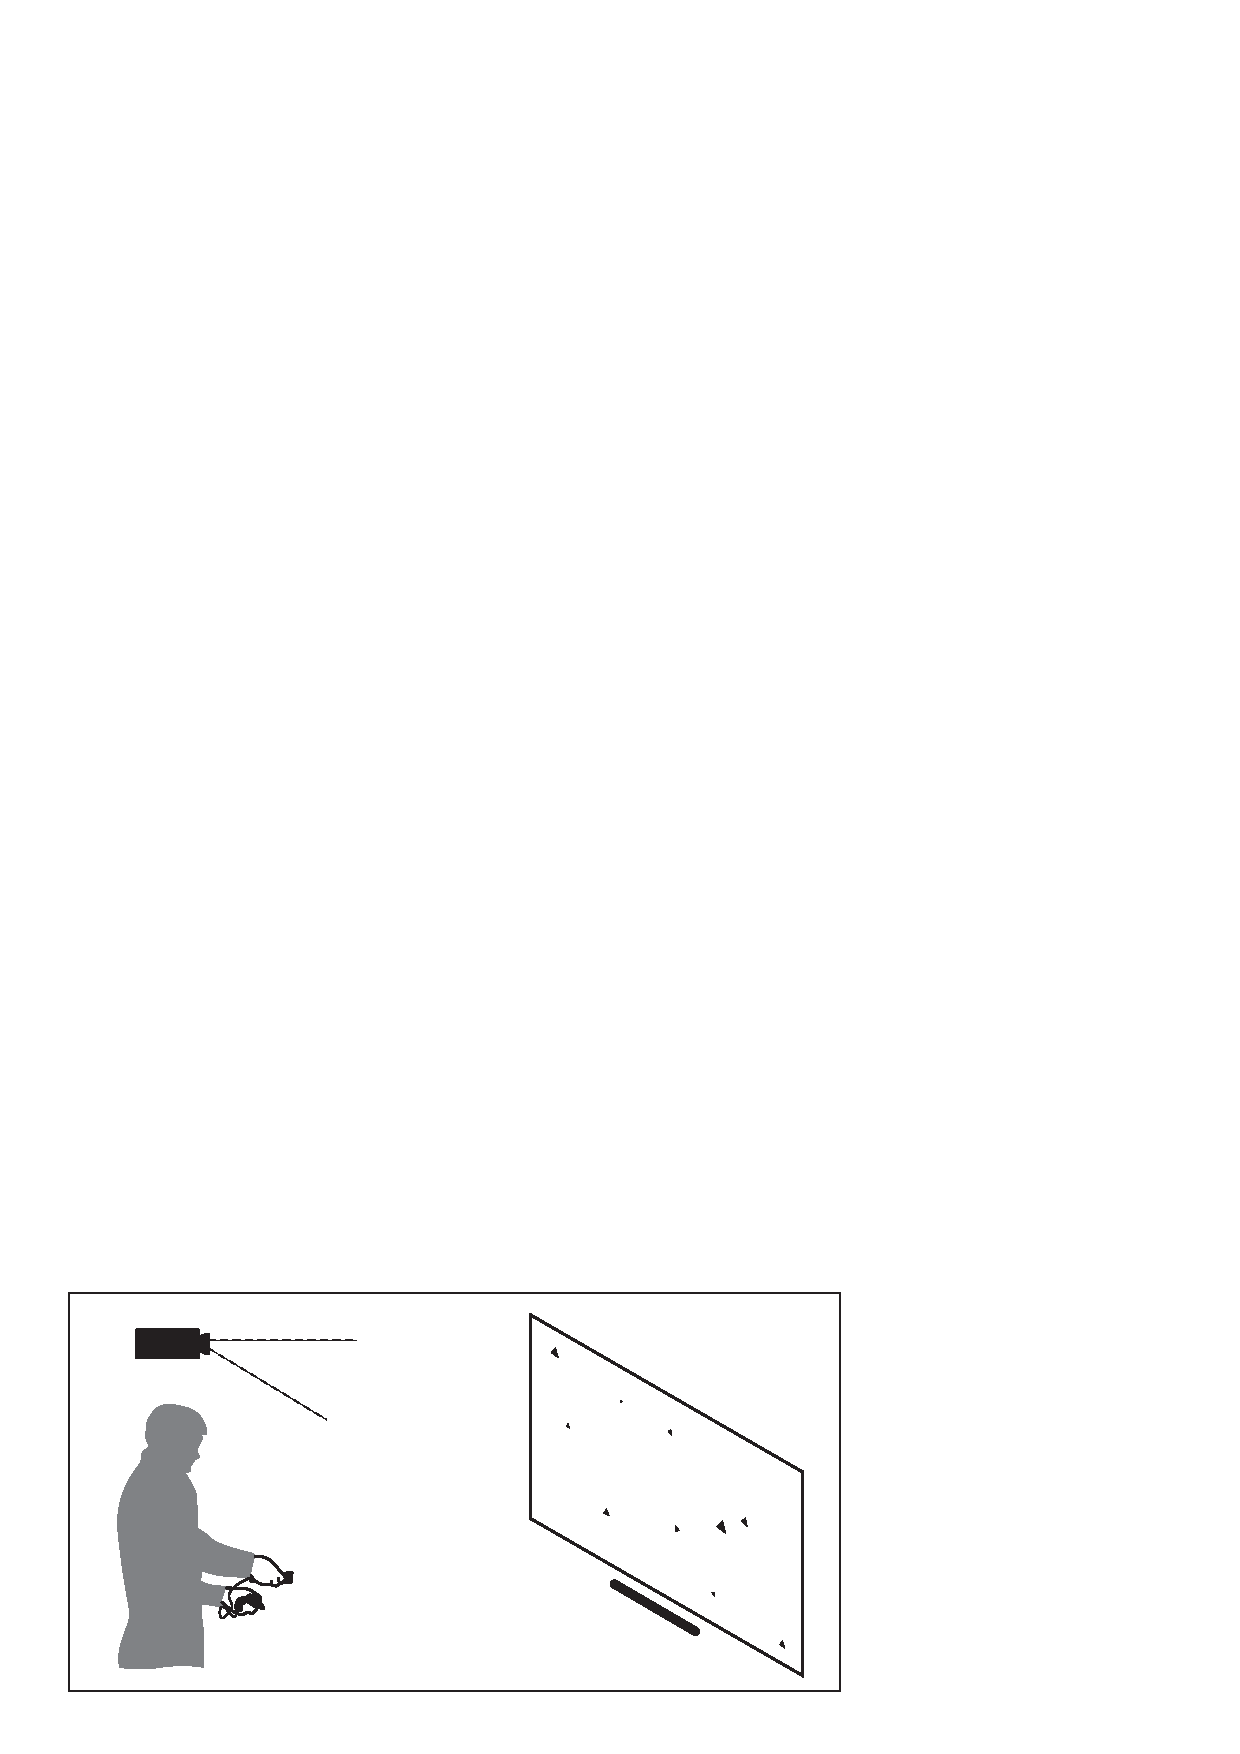
\includegraphics[width=0.7\columnwidth]{img/setup}
\caption{Standard set up of Sputnik}
\label{fig:sputnik-setup}
\end{center}
\end{figure}




\subsection{The Virtual Scene}

\begin{figure}[hbtp]
\begin{center}
\subfigure{
	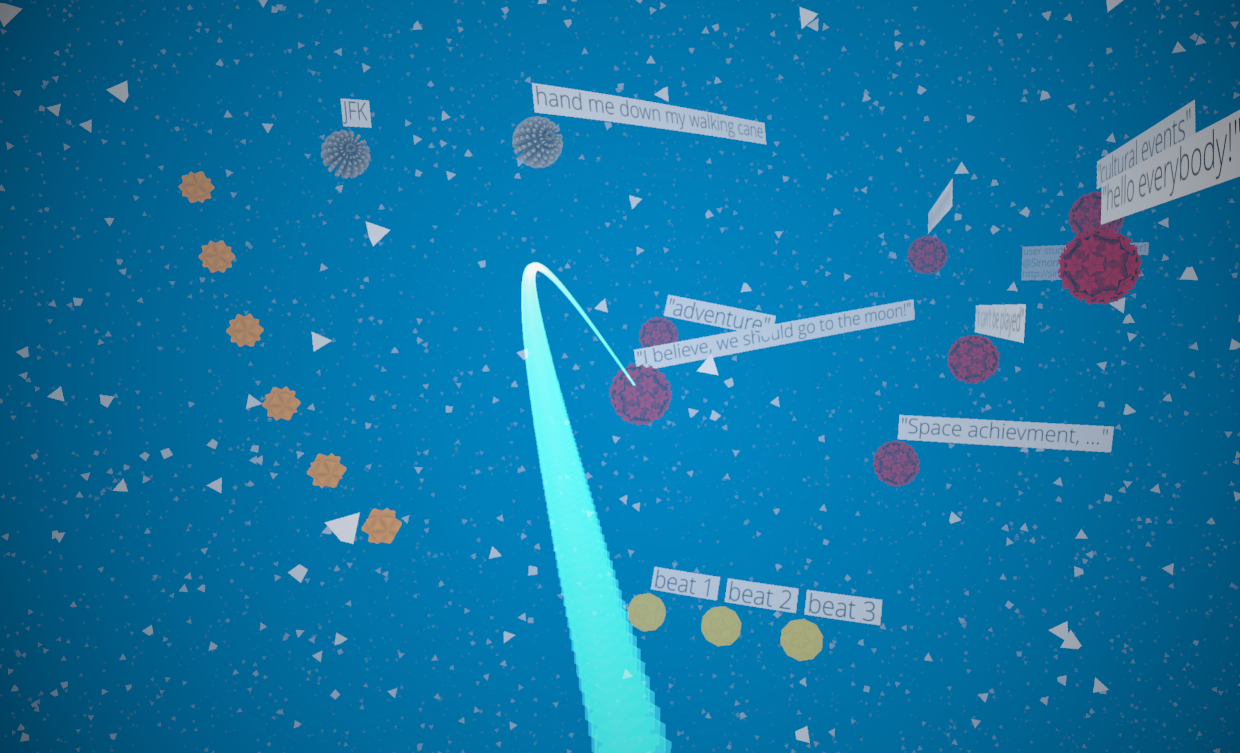
\includegraphics[width = 0.45\columnwidth]{img/screen-shot-all}
}
\subfigure{
	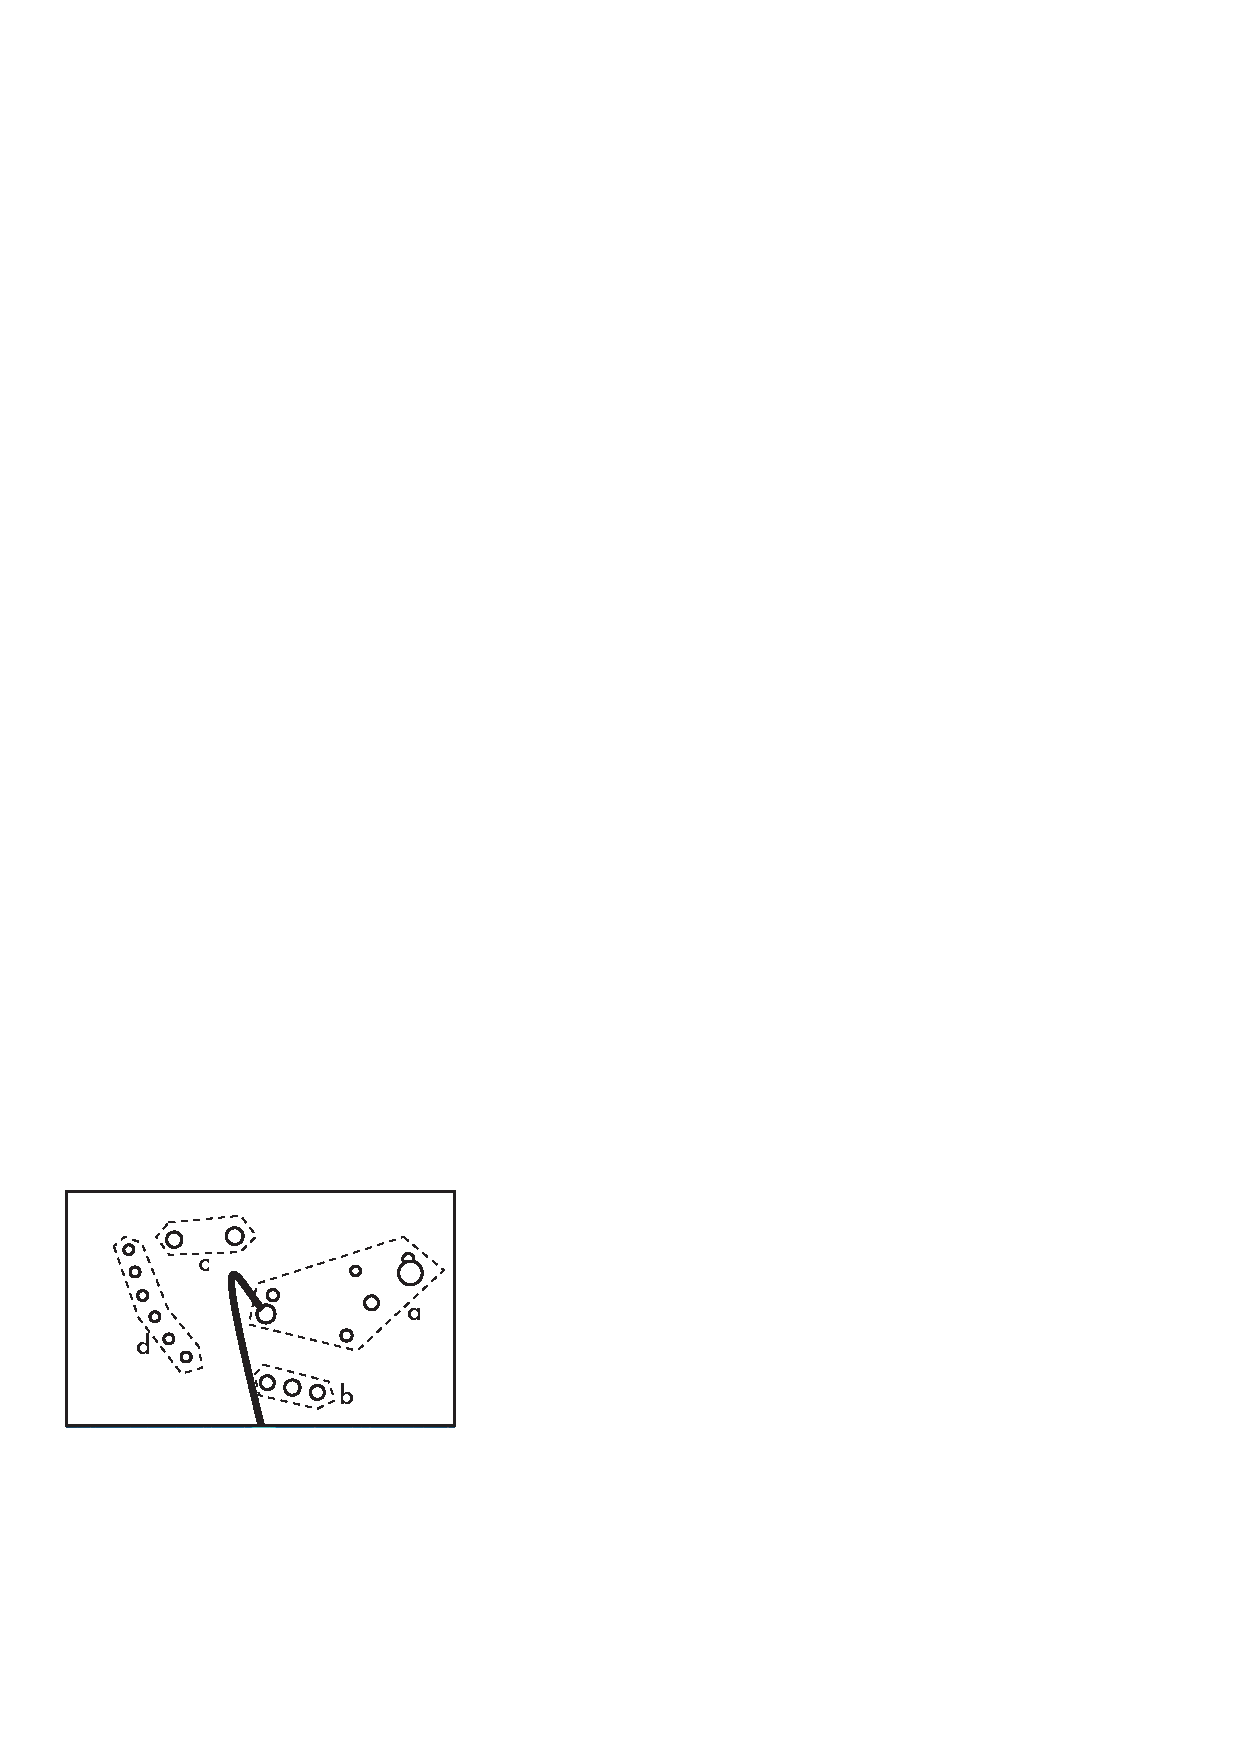
\includegraphics[width = 0.45 \columnwidth]{img/overview-illu}
}
\caption{The objects in the scene: (a) Samplers, (b) Players, (c) Tape Machines, (d) Harmonic Harp}
\label{fig:screen-shot-overview}
\end{center}
\end{figure}


Figure \ref{fig:screen-shot-overview} shows an overview shot of sputnik. The svirtual cene consists of the following parts:
\begin{enumerate}
\item The light blue and bent \emph{arc of light} starting in the middle of the lower edge and going \emph{into} the picture. It is directly controlled by the user and is the primary mean of interaction.

\item Objects the user can interact with: sampler (red), player (yellow), tape machine (grey), harmonic harp (orange)

\item Textual labels on the interactive objects. Each label contains a short text or name describing the interactive object. Figure \ref{fig:sampler-labels} shows a few \emph{samplers} with their labels.

\item Randomly generated star field. It is not interactive and static. It serves an aesthetic purpose as well as providing important reference points for the users orientation.

\item Coloured Fog. The fog provides depth cues for the objects
\end{enumerate}

\begin{figure}[hbtp]
\begin{center}
\subfigure{
	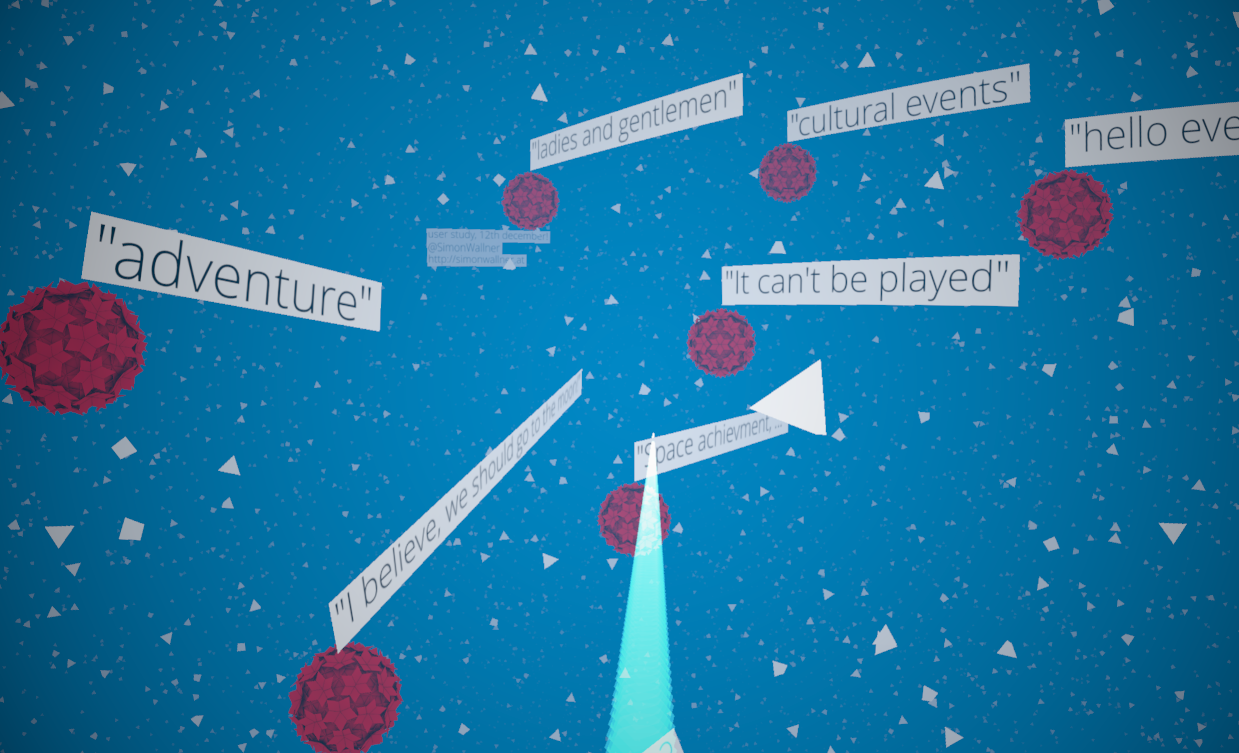
\includegraphics[width = 0.45\columnwidth]{img/screen-shot-sampler}
}
\subfigure{
	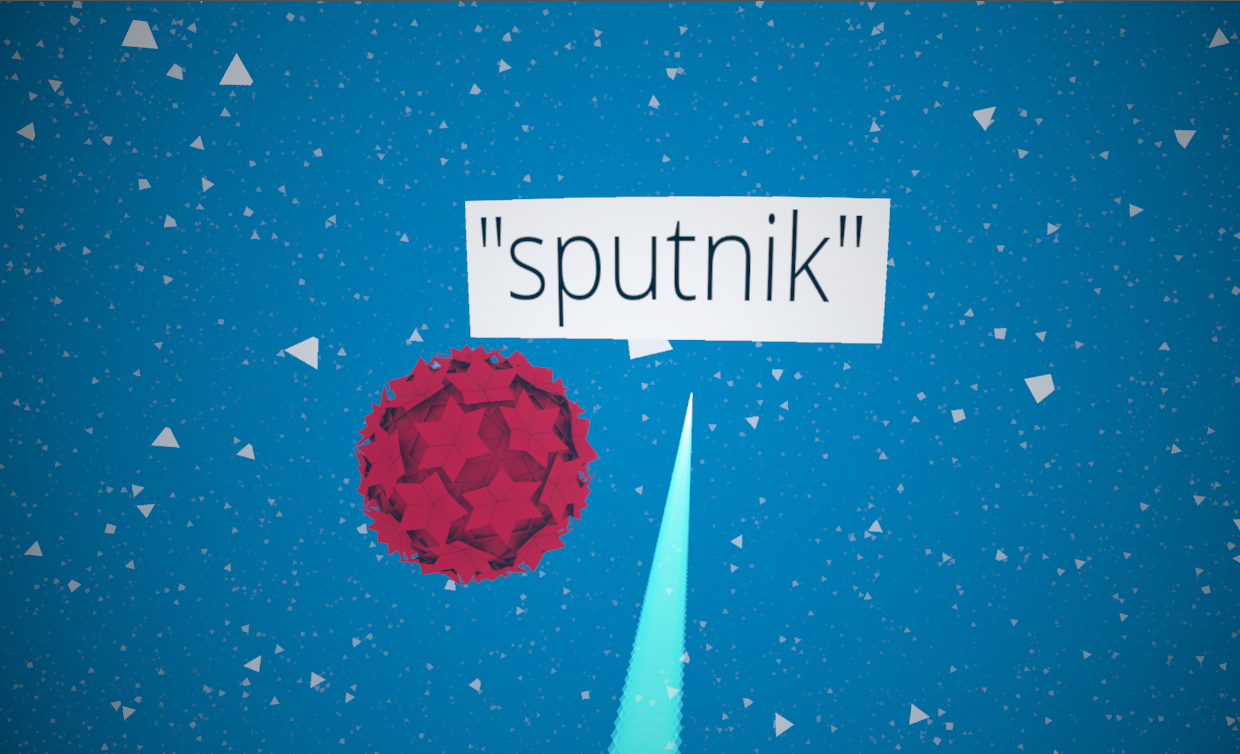
\includegraphics[width = 0.45 \columnwidth]{img/screen-shot-label}
}
\caption{A group of \emph{samplers} and the close up of a single \emph{sampler} with their attached labels}
\label{fig:sampler-labels}
\end{center}
\end{figure}


The visual representation of Sputnik serves a dual purpose. On the one hand it is the sole graphical interface for the user and on the other hand it should be visually pleasing for the audience and allow them to understand the process of music creation in a live setting. Common music software usually focuses on the performer, leaving the visual performance in most cases to a dedicated and specialised VJ. Sputnik tries to bridge this rift by using the visual representation both as an interface to the performer and the audience. 

% add: visual expression, just like VJing...

The textual labels in Sputnik are aimed at both the performer and the audience. The text on the labels is hard coded and does not change during run time. It can be used to convey additional information to the performer about a certain object, but it can also allow the audience to gain more information about the piece. The function of the objects can become clear even if the object is not currently in use. This can also introduce an element of anticipation when an object with a certain label is visible but the performer does not yet interact with it.





\subsection{Navigation and Camera Controls}
Sputnik is controlled from a first person perspective. The user can navigate the scene by pushing the Nunchuck's analogue stick in the respective direction. Pushing the stick forward moves the camera into the scene, pushing it to the left moves the camera to the left and vice versa.

Tilting and panning is controlled by pointing the Wiimote to the top/bottom/left/right of the screen. The farther it is pointed away from the neutral center position the faster the camera movement is. Figure \ref{fig:sputnik-navigation} illustrates the navigation.

Sputnik's camera uses a fixed \emph{up direction}. The fixed up direction is commonly seen in cinema and video games, even though it is not intrinsic in the space inspired setting. It furthermore should limit the camera's degree of freedom and make it more accessible.

\begin{figure}[hbtp]
\begin{center}
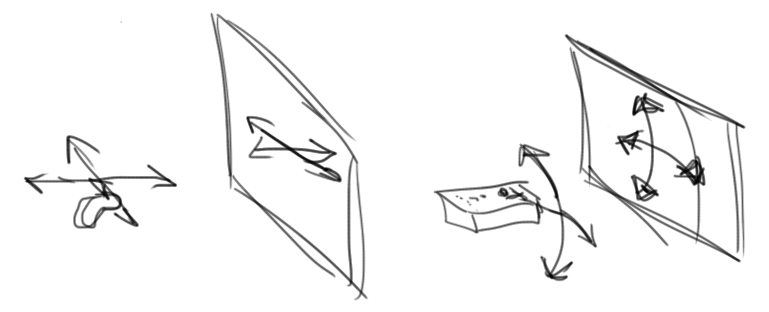
\includegraphics[width=0.85\columnwidth]{img/navigation}
\caption{The Nunchuk's analogue stick controls the camera's dolly and track movements, the Wiimote's IR pointer controls the camera's tilt and pan movements.}
\label{fig:sputnik-navigation}
\end{center}
\end{figure}



\subsection{Interaction}

\begin{figure}[hbtp]
\begin{center}
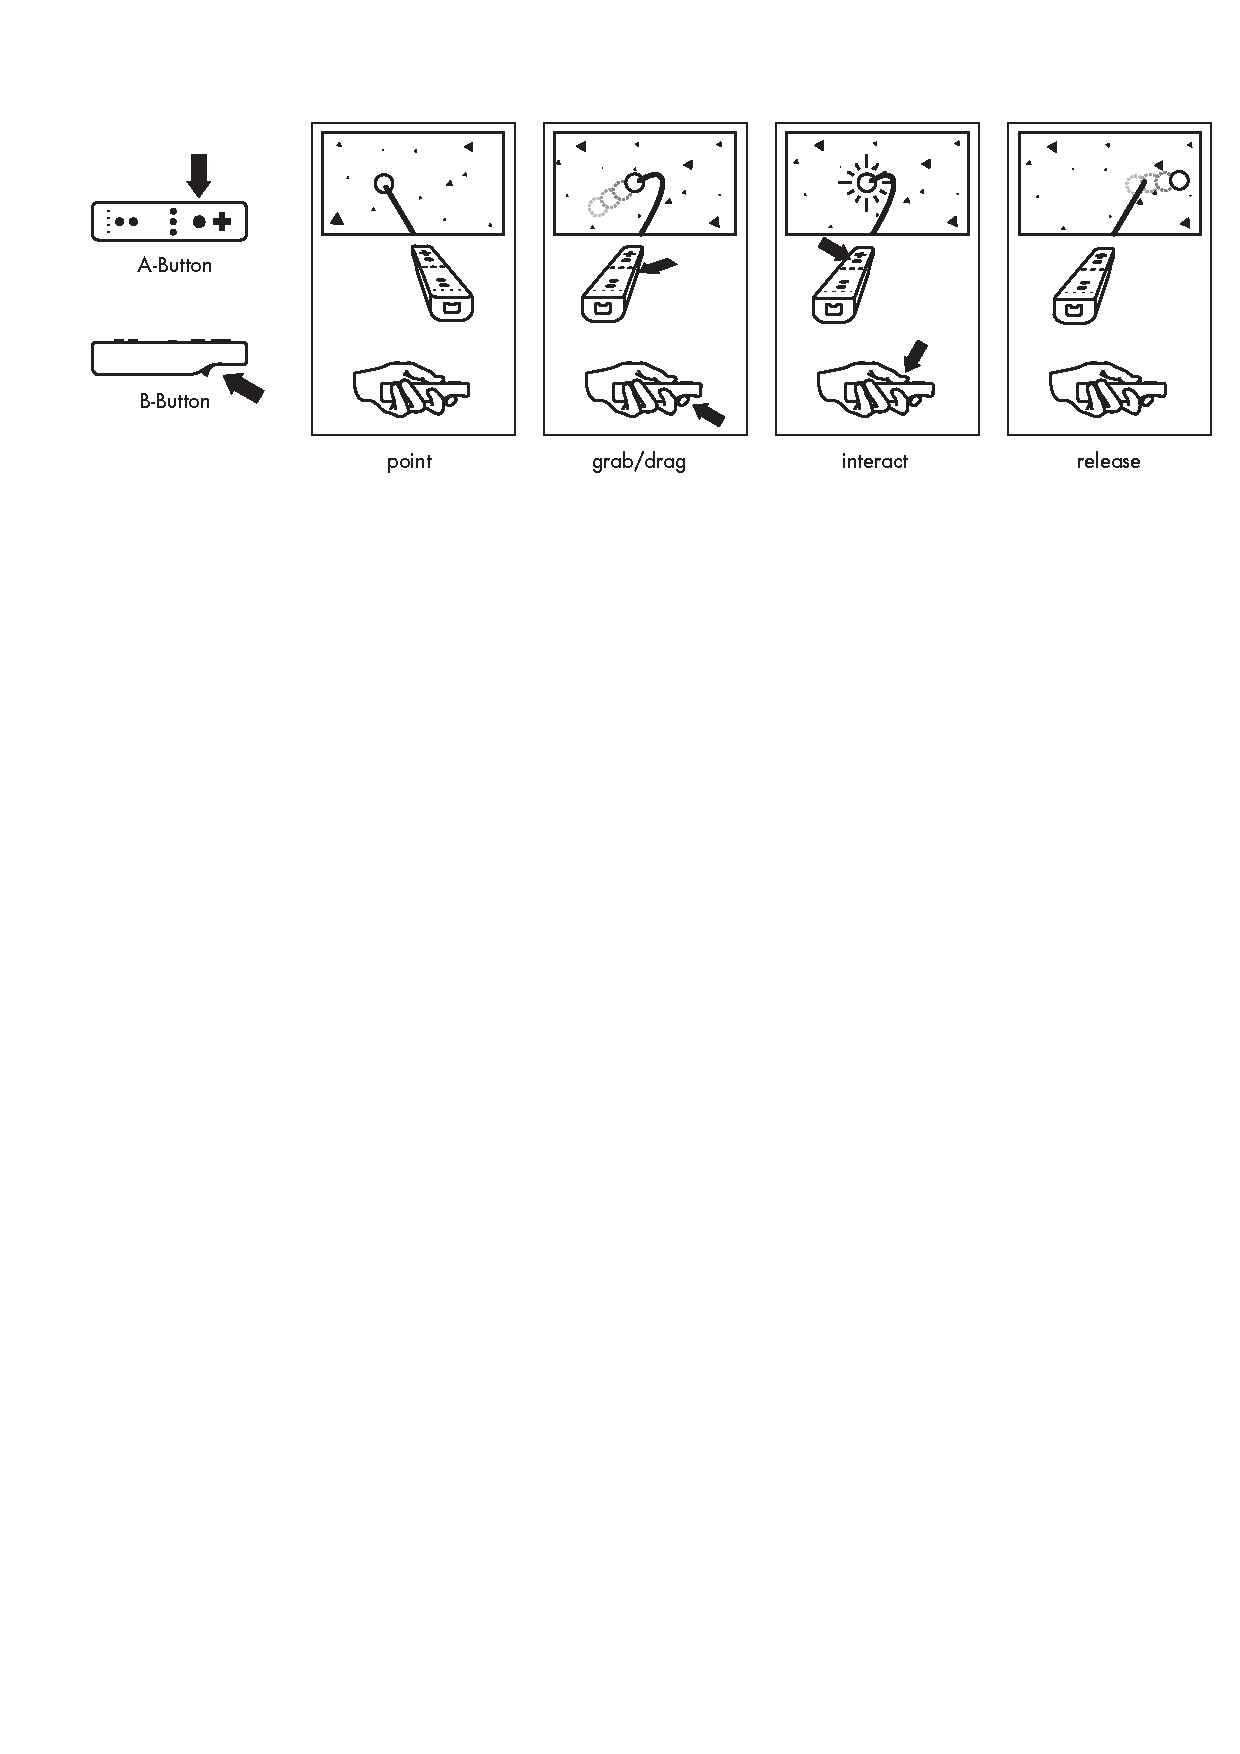
\includegraphics[width=0.95\columnwidth]{img/sputnik-overview}
\caption{The basic interaction vocabulary of Sputnik}
\label{fig:sputnik-overview}
\end{center}
\end{figure}

Figure \ref{fig:sputnik-overview} illustrates the basic interaction vocabulary of Sputnik. The user can interact with the scene via an \emph{arc of light} metaphor. It seems as if the arc of light was coming out of the Wiimote and reaches into the scene, acting as a bodily extension of the user into the virtual space. Through this \emph{arc} the user can \emph{point} at objects, \emph{grab} them and also \emph{drag} them around the scene.

Interactive objects behave in a simplified physically plausible way, each featuring distinct weight and friction. Dragging objects causes the arc to bend like a fishing rod, reflecting the physical properties of the object.

Each interactive object in the scene can react individually to user interaction. The following classes of objects currently exist in Sputnik:

\begin{description}
\item[Sampler (red)] The \emph{sampler} object reacts to the press of the \emph{A button} while it is grabbed. While the button is held a preloaded sample is played in a loop and stops immediately when the button or the object is released. Playback always starts at the beginning of the sample.

\item[Player (yellow)] The \emph{player} object reacts to the press of the \emph{A button} while it is grabbed. Pressing the \emph{A button} starts and stops the playback of a preloaded sample. It is not automatically stopped when it is released. Playback is looped and always starts at the beginning.

\item[Tape Machine (grey)] Modelled after an old tape machine and inspired by \emph{musique concrète} the \emph{tape machine} object controls the play back speed of a preloaded sample via the object's movement speed in the virtual space. The faster it moves the faster the playback. Playback is looped.

\item[Harmonic Harp (orange)] The orange spheres form a kind of \emph{harmonic harp}. Each sphere controls a single sine wave oscillator and the volume is determined by the the sphere's distance to its origin. Additionally the spheres are pulled towards their respective origins by a constant force that is linear in the distance from the sphere to its origin. The oscillators are tuned to the natural harmonic series which makes them easy to play with and avoids dissonances.
\end{description}

Each interactive object is preloaded with a different sample or sound in an external application. By interacting with the different objects and arranging them in the virtual scene, users can create musical performances that are both musically and visually expressive.


\subsection{Simplified Physics}
Sputnik uses simplified physics simulations to give the interactive objects their distinct physical properties. An object's properties are described by \emph{mass}, a \emph{movement vector}, as well as a movement \emph{damping constant}. SI units are used unless otherwise noted.

The dragging force of the arc on an object is linear in the distance from the object to the intersection of the unbent arc with the plane that goes through the object, with a normal pointing at the camera. This intersection point also defines the direction of the force vector.

In each frame, the speed of an object is then computed as 
\begin{equation}
v_i = v_{i-1} + \frac{F * \Delta t}{m} 
\end{equation}
where $v_i$ is the object's movement vector in frame $i$, $F$ is the current force, $m$ is the mass and $\Delta t$ is the frame time. Force is only applied at the center of the objects, and thus never causes a rotation of the object.

Damping of the object's movement is implemented by a simple exponential decay, given as
\begin{equation}
v_i = v_{i-1} * e^{-\lambda * \Delta t}
\end{equation}
where $\lambda$ is the damping constant.



\subsection{Creating sound}
Sputnik's interactive objects individually react to the users input and use the MIDI protocol to communicate with an external application. Sputnik itself does not create any sounds. Sound creation is handled entirely by an external application.

Thanks to the simplicity and the pervasiveness of this protocol, virtually every music software can be used together with Sputnik. In the current set up \emph{pure data (pd)}\footnote{\texttt{http://puredata.info/}} is used for sound creation. A simple patch is used that builds on \emph{boctok-1}, a small collection of pd patches written by the author prior to this project. 

Communication is only one way; from Sputnik to the external application. The MIDI channel and controller number every object uses is currently hard coded into Sputnik an can only be changed in the source code. 


\section{Implementation}
Sputnik is implemented in C++ with Mac OS X as its development platform. The project is split into two sub projects: The special purpose Sputnik and the more general purpose \emph{kocmoc-core}. Kocmoc-core provides core services that are then used by sputnik to build the final system. Some code of kocmoc-core existed prior to this project, but most of it was created in the course of the project. 

The source code of both Sputnik and kocmoc-core is licensed under the permissive MIT open source license and is publicly available on github\footnote{\texttt{https://github.com/SimonWallner/sputnik}} \footnote{\texttt{https://github.com/SimonWallner/kocmoc-core}}.

Sputnik uses OpenGL 2.1 with a few extensions to display the virtual scene. The renderer is fairly simple and displays unlit, textured objects with baked ambient occlusion maps. The computation of the homogeneous fog is realised in the vertex and fragment shader and a post processing effect is applied. This effect adds a barrel distortion to compensate the wide field of view and vignetting. A simple form of full screen anti aliasing is also added in this stage.


The \emph{Assimp}\footnote{\texttt{http://assimp.sourceforge.net/}} and \emph{devIL}\footnote{\texttt{http://openil.sourceforge.net/}} libraries are used to load assets. Font rendering is implemented using the \emph{freetype}\footnote{\texttt{http://www.freetype.org/}} library.

\emph{RtMidi}\footnote{\texttt{http://www.music.mcgill.ca/~gary/rtmidi/}} is used to send MIDI messages to external applications and \emph{WiiC}\footnote{\texttt{http://wiic.sourceforge.net/}} was used to interface with the Wiimote and Nunchuck controller.

Figure \ref{fig:flow} illustrates the data flow in the main run-loop. First, the devices are polled, which causes input callbacks to be fired. The components are subsequently updated and finally the scene is sent to the renderer.


\begin{figure}[hbtp]
\begin{center}
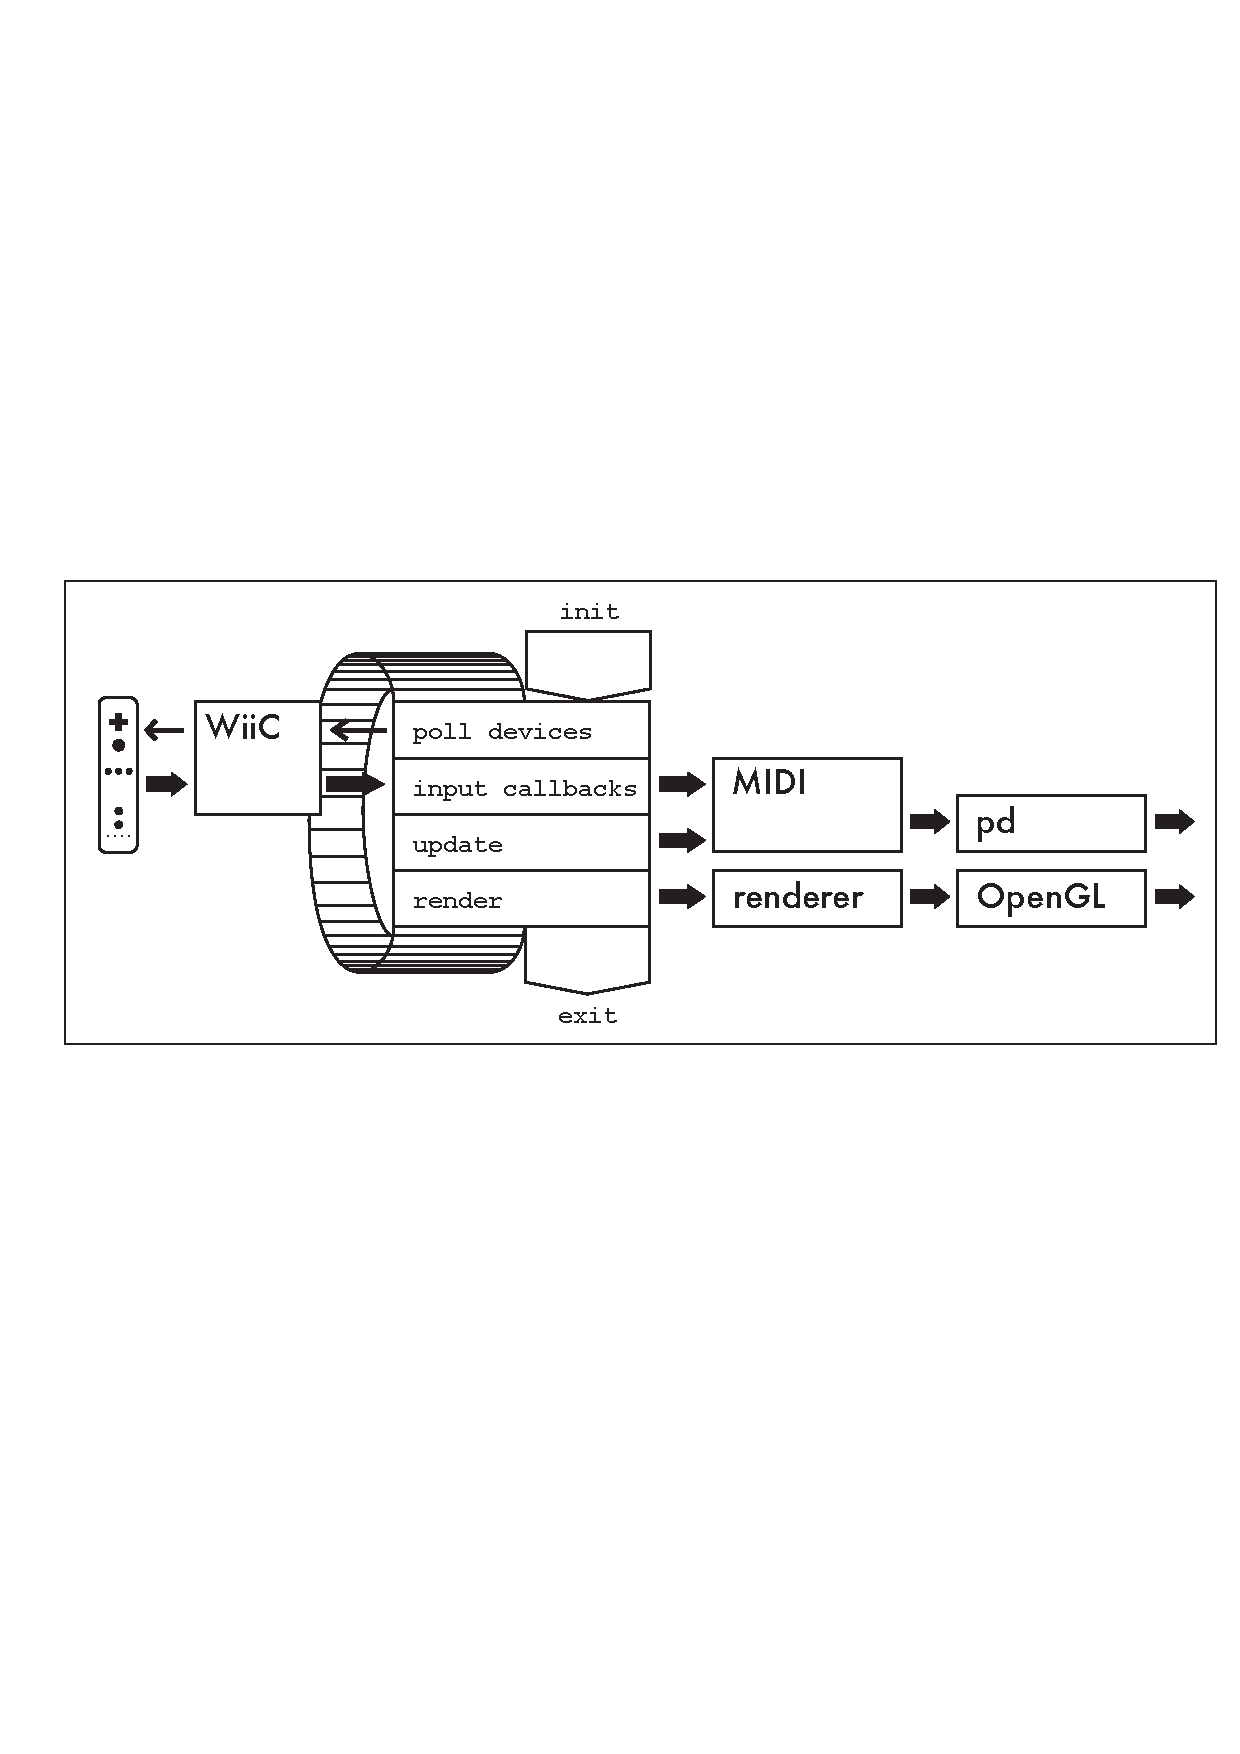
\includegraphics[width = 0.95 \columnwidth]{img/flow}
\caption{The data flow in the run-loop.}
\label{fig:flow}
\end{center}
\end{figure}





\section{Wiimote Input}
The Wiimote controller was chosen for its pointing functionality as well as the motion sensing capabilities, even though they haven't been used in the final project. The accompanying Nunchuck controller was also used to allow the standard analogue stick driven navigation.

The Wiimote has an built in low resolution IR camera and its feed is directly processed on chip. The feed itself is not accessible but data of up to 4 tracked IR points can be read. the Wiimote's update rate is reported to be $100Hz$ which gives an lower bound for the worst case lag of $10ms$. The used Wiimote library takes care of most of the processing and conveniently returns the computed pointer location in relative screen coordinates.

A drastic constraint of the Wiimote's IR pointer however is the relatively narrow field of view. It is very easy to leave the small sensing area. During the development it turned out that using the Wiimote for the tilt/pan movements of the camera can alleviate this problem a little. Users seem to intuitively try to compensate the camera's rotation, thus maintaining a focus on the neutral area in the center of the screen. Without it users easily lost the focus an had troubles finding \emph{back onto the screen}.

The used Wiimote library supports more than one Wiimote and the input system in Sputnik would also support multiple input devices at the same time. The option to \emph{dual wield} two Wiimotes and to interact with two arcs of light simultaneously was given up in favour of the more standard analogue stick track/dolly controls, that allow the users to easily navigate the scene. 





\section{The Arc Of Light}
The arc of light forms the foundation of Sputnik and is its core contribution. It acts as a bodily extension of the users body into the virtual scene. Through the arc the user can use the interaction vocabulary described above. It has the following behaviour.

If no object is grabbed, the arc follows the user's input directly. This input is not filtered and is used directly \emph{as is}. This introduces a slight jitter but on the other hand does not take away from the system's responsiveness. 

Low pass filtering however is desired in most scenarios and is indirectly implemented via the physical properties of the interactive objects. The higher the weight of the object for instance, the stronger the filtering is. while grabbing an object the arc bends accordingly to the the physical properties of the object and the dragging force of the user. It bends like a fishing rod, a natural metaphor that seems to readily understandable to the users.

One of the core advantages of the arc is that even very strong filtering can be achieved without making the system feel laggy and slow. It happens in a way that is transparent and understandable for the user, and in a informal user study the testers reported that the system is very responsive.



\section{Mapping the System}
What further distinguishes Sputnik from other projects or interfaces, and a commonality it shares with some tangible interfaces, is the spatial component. Users can move the interactive objects in 3D space in a meaningful way.

The spatial arrangement of objects can be reconfigured at run time. This allows the performer to create new configuration during the performance. 

For the objects that react to their position of movement the spatiality is mapped directly to the sound creating application. The \emph{tape machine} for instance maps its movement speed to the playback speed of the sample and the \emph{harmonic harp} maps the distance of its spheres to their respective origins to the volume of each oscillator. These are mappings that cannot be achieved by a conventional hardware interface. The informal user study also hinted, that these mappings where the most interesting and novel ones.



\section{Evaluation}
\label{sec:evaluation}

\subsection{Method}
Sputnik was evaluated in a small and informal user study with only three participants. The testers where asked to use Sputnik and a small questionnaire and interview where held afterwards. Sputnik was tested with only one person at a time.

Due to the very small number of participants this study can only be seen as a precursor to fully fledged user study. A relatively wide range of questions and topics was used in the evaluation to gain a broad overview about how Sputnik is used, what general problems arise, and how suitable it is as an interface for musical expression.

The whole test was recorded on video and the interview afterwards was audio recorded for later analysis.

\subsection{Participants}
Only 3 participants (all male) took part in the test, with an average age of 26 (SD = 5.2). All had a musical background having played classical instruments but not on a professional level. Two had additional experience with computer and sample based music.

None of the participants had used a Wiimote prior to the study, all where right handed and colour normal.

Two participants have seen short explanatory demo videos of Sputnik that where used in order to find participants.

\subsection{Set Up}
The test was conducted in a darkened room with the participant standing about 4 meters away from the overhead projected screen with a diagonal of about 2 meters. The screen had an aspect ratio of about 16/9 and the screen's center was about 1.5m above ground.

The Wiimote sensor bar was positioned a few centimetres below the lower edge of the picture. A small stereo speaker set was used that was located on the floor right behind the participant.

\subsection{Procedure}
At the beginning of the test, participants where asked for basic statistical data. The testers where informed about the test plan and the controls where briefly explained. 

The first task was to try out the navigation and familiarise with the controls. This included basic navigation and orientation as well as grabbing and interacting with objects. 

In the second stage, participants where asked to describe for every class of interactive objects, what they do and how they react to user interaction.

The third stage consisted of a brief impromptu musical performance. Time was given to plan and structure it in advance and participants where asked to start when they felt ready. The length of the performance was not specified, only a vague rule of \emph{not too short, not too long} was given.

The test was concluded with a brief ordering task. The participants where presented with four objects and where asked to bring them in order according to their weight. Those objects did not create sounds.

After the practical test, a one-page questionnaire consisting of 4 5-point Likert-items and 7 questions inspired by QUIS\cite{Chin1988}. A short interview guided by a set of pre-written questions was conducted afterwards.

The questionnaire and interview form can be found in the appendix. \ref{} \ref{}


\subsection{Design}
The answers to the Likert items are discussed individually and mean and standard deviation values written as mean/SD are given for the QUIS section. Since linearity of the scale in the QUIS items cannot be assumed, calculating mean and standard deviation is not correct. Also the very low number of samples speaks clearly against it, however it is a convenient way to look at the data.



\subsection{Results}
Overall reactions to Sputnik were rather positive which is hinted in the results of the QUIS inspired questionnaire seen in figure \ref{fig:QUIS}. Due to the small number of participants no direct and strong conclusions can be drawn from this evaluation and it should rather be taken as a hint on what Sputnik does good, and where there is more room for improvement.

\begin{figure}[hbtp]
\begin{center}
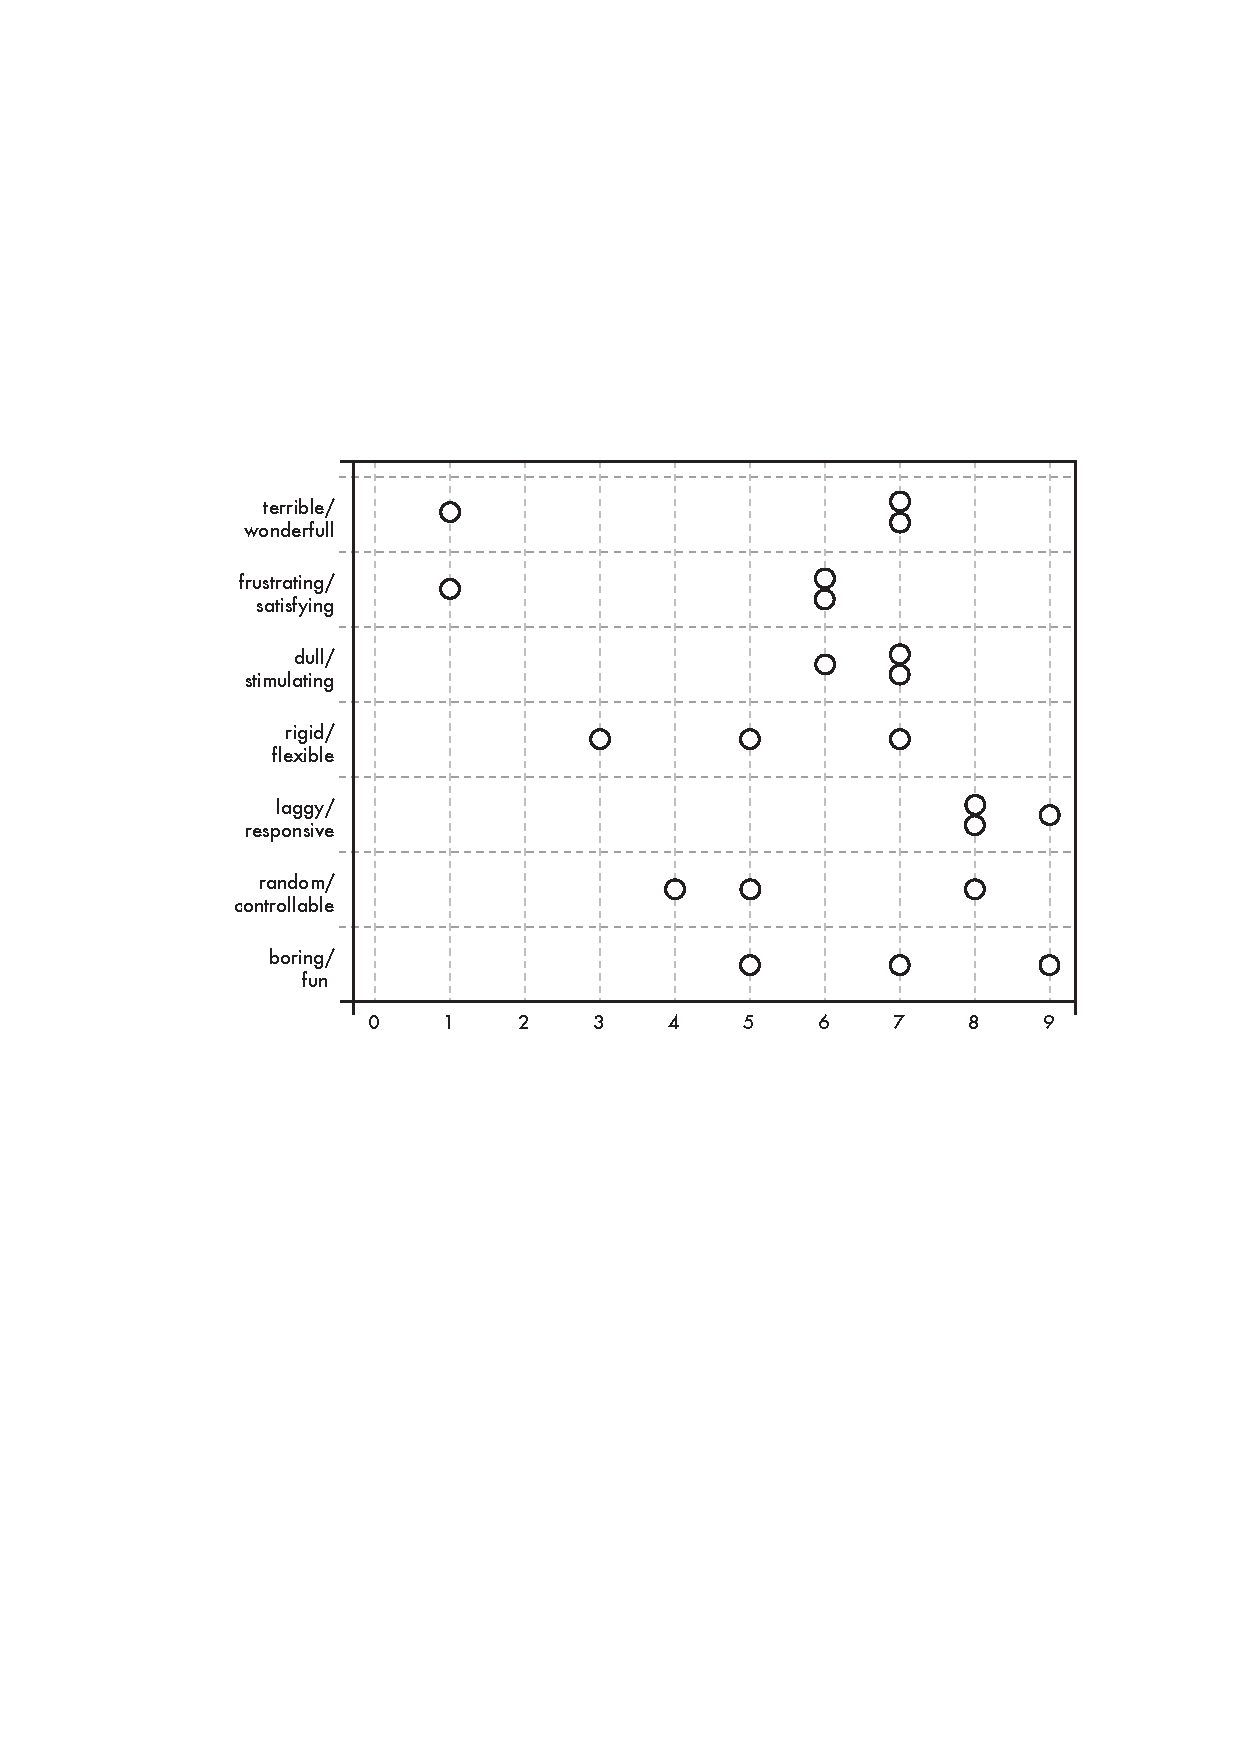
\includegraphics[width = 0.8 \columnwidth]{img/stripchart}
\caption{QUIS results...}
\label{fig:QUIS}
\end{center}
\end{figure}

Unfortunately, the results of the Likert items where inconclusive: The first question, "Sputnik is easy to use" resulted in the answer triple (strongly disagree, neutral, agree) and all other items resulted in (disagree, neutral, agree).



% # controls and navigation
% - no prior wiimote experience. could use it quite well. lost focus a few times, 
% - narrow FOV
% - no precise control --> jittering, sensitivity?
% - grab accuracy
% - lack of movement/sophisticated movement/motion patterns
% - pull missing, mentioned 3 times
\subsubsection{Controls and Navigation}
Even though none of the participants had prior experience with the Wiimote, all managed to effectively use Sputnik during the test. After only a few moments the participants where able to navigate the scene and interact with the objects. 

A problem however was the narrow field of view (FOV) of the Wiimote, resulting in uncontrollable camera movement if the sensor bar is not in the Wiimote's FOV. During the test this happened about 3-5 times per participant.

Another problem was insufficient pointer precision. All participants struggled at least once trying to grab small or faraway objects. This could partially be explained by the slight jitter of the Wiimote's pointer and it's narrow FOV, that requires rather subtle movements.

Differences in movement patterns could also be observed. Two of the three participants did not move the camera very often. Phases of interaction (rotate, grab, interact) and camera movement were clearly separated and camera movement was rather erratic. The third participant also begun in a similar fashion but then gradually started to combine movement and interaction into more sophisticated movements like \emph{circle strafing} (moving sideways while turning) and moving while dragging an object.

All participants tried to pull objects by grabbing them and moving backwards at the same time. This is not implemented in Sputnik and this was noticed and explicitly mentioned by all participants during the test.



% # visual
% - missing visual feedback from the objects
% - visual rep no meaning, interactive star field
% - no read labels
% - use pointer to direct gaze, or when talking
\subsubsection{Visual}
All participants where missing feedback of the interactive objects regarding their musical state, e.g. a way to see if a player object was playing or not. One participant mentioned explicitly that the visual representation has no meaning, stating that: "[...] objects and their forms, and so on..., didn't make any sense". Answering another question he also mentioned that it would be more interesting if also the star field was interactive and reacted to the music performed.

The participants seemed to not pay much attention to the textual labels of the objects. The labels have a fixed orientation and the camera was often in a position from which they were not readable. This can be related to the rather simple navigation patterns mentioned above and that the effort to move the camera in a position from which the labels were readable was to high.



% # interaction
% - participants found out what objects do and how they react.
% - artificial distance limit
% - controller waggle
% - participants seemed to have no troubles using the arc
% - responsiveness --> Filtering, lag
% - direct/quick access to stuff
% - use of space, spatiality
% - dragging of all objects, even samplers and stuff. --> natural affordance of the system?
\subsubsection{Interaction}
All participants could deduce the functions of the sampler and player objects. Descriptions of the tape machine and harmonic harp were not as precise but captured their general mode of operation. 

Participants seemed to have no problems using the arc and all participants responded positively when being asked about immersion into the scene. One participant even said at the end that: "I liked the link from me to the objects,.. when you hold the objects. It made sense". A point noticed and mentioned by all participants was the arbitrary distance limit of the arc. Objects could only be grabbed if they where inside a certain range.

Two of the 3 participants also tried to waggle the Wiimote, a gesture which is not directly used in Sputnik. 
 
In regards to the samplers all three participants indicated the need for a way to quickly and directly access some of the objects to either have certain sounds available all the time or to quickly change between sounds.

Even though Sputnik was not running at a very high frame rate during the test (~30-40fps) participants indicated in the QUIS that it was \emph{very responsive} and no comments about lag where made in the following interview.



% # improvisation/objects
% - spatial arrangement of objects prior to performance
% - similarities in the performance
% - the objects
% - models
% - interesting objects, harp, tape

\subsubsection{Improvisational Performance}
All participants used a similar pattern for their improvisation, alternating between the different groups of objects. The participant without prior experience with computer and sample based music had trouble putting together a coherent performance and seemingly disliked the task

The two users with experience in computer and sampler base music, arranged the objects before the performance and seemed to be \emph{planing ahead}. A procedure that is probably similar to how they would approach such a task with their usual set up and tools.

Likeability of the interactive objects seems to correlate with the amount of interactivity they provide and how it is used in the system. The tape machine and harmonic harp generally received better comments than the sampler and player objects. Two participants said, that they disliked the player object for being uninteresting and lacking interaction.


% # weight test
% - continuous grab
% - weight metaphor
\subsubsection{Object Sorting}
Two participants sorted the objects correctly, one brought the lightest two in the wrong order. All participants used a continuous grab to assess the weight of the objects. During the development another user tried to \emph{throw} the objects to observe their weight, but this behaviour was not observed in this study.

% # meta
% - exchange sounds/customise
% - fatigue in shoulders
\subsubsection{Misc.}
All participants expressed the need to exchange the sounds and fit Sputnik to their needs in order to be useful in a live setting.

One participant reported fatigue in his shoulders, an aspect of Sputnik that was not accounted for in the study, but is probably an important factor in real world usage scenarios.






\section{Discussion and Conclusion}
\label{sec:discussion}
% interpretation of the user study
%	- is it any good
%	- ease of use, easy to pick up
%	- motion patterns --> training, advanced techniques
%	- lessons learned about "instruments"
%	- arrangement of objects prior to performance

The user study indicates that Sputnik is relatively easy to pick up and use, even for users with no prior experience with the Wiimote controller. More sophisticated and advanced movement patterns seem to emerge as the participants grow accustomed to the system.

The arc of light worked well in providing a bodily extension of the user into the virtual scene. It can be effectively used in combination with physical objects to low pass filter user input without loosing the perceived responsiveness of the system.


% Tangible Interface, 
%	- UI unification, i.e. harmonic harp
%	- coupling of action and perception space
%	- even though not physical, tangible can be in close relation
\cite{Sharlin2004} introduced the concept of \emph{spatial TUIs}, TUIs that feature a strong spatial component. Sharlin et al. elaborate on \emph{UI unification}, the tight coupling and unification of the action and perception space. Even though Sputnik is not a TUI, a strong relation to this field exists.

The tape machine and harmonic harp in Sputnik employ strong UI unification. Input and output are tightly coupled through their virtual representation and cannot diverge. Furthermore, their spatial configuration is directly mapped to the sound parameters. By seeing Sputnik as a \emph{virtual TUI} with the arc of light as a bodily extension of the user into the virtual space, existing TUI literature can be used to study and evaluate Sputnik. Conversely, translating actual TUIs into a virtual environment can open up new viewing angles on them.

	
% Musical expression?
The question of musical and visual expressiveness can not be answered through this evaluation. More time needs to be given to the participants and more possibilities to customise Sputnik to their needs and musical and visual style. An approach similar to the one used in \cite{Gurevich2010} could be a good starting point for further evaluations.

% Wiimote not very practicable --> PS move
What the user study very clearly showed is that the Wiimote is not very suitable as a controller for Sputnik, due to its narrow field of view. It is too easy to move out of the FOV resulting in a loss of control over the camera. users can usually recover within a few seconds, but still this would be a show stopper if used in an actual live performance. Other Input devices like the Playstation Move\footnote{\texttt{http://en.wikipedia.org/wiki/PlayStation\_Move}} controller or Microsoft's Kinect\footnote{\texttt{http://en.wikipedia.org/wiki/Kinect}} should be evaluated as an alternative.


\section{Future Work}
% impact on audience, what do they think
% customisable for artists --> scripting
% arc of light for other applications
% increase performance to >60fps
% more advanced controls --> waggling, % dual wield
% develop a comprehensive piece of music to test creative limits
% commonalities and differences to TUIs
% visual feedback to sound

This project raised a lot of questions and opened up many directions for future work:

Sputnik's impact on a live audience and how it can be used for visual expression should be explored. This is an important aspect of Sputnik and a larger scale study is needed.

To be useful for artists and users with less of a technical background scripting should be included to allow the artist to change the scene, create new objects and models and change the input/output mapping. Additionally the performance should be increased to run at $> 60fps$ for a smoother experience.

More advanced controls like waggling and other motion based controls should be evaluated inside Sputnik. Also the option to use a second Wiimote instead of the Nunchuck and the therefore arising interaction possibilities should be explored and evaluated.

Direct visual feedback of the interactive objects to the generated sound should be implemented. The lack of it was mentioned by all testers and it might also be crucial for the effect on a live audience. Additionally a musical possibilities should be explored by devoting the time and creativity to create genuine pieces of music for Sputnik and performing them live.

The arc of light metaphor should be further explored in other fields outside the domain of musical interfaces. 



\section{Acknowledgements}
I would like to express my greatest thanks to my supervisor Esben Warming Pedersen, who always turned me into the right direction and helped me in finding and refinding the project's focus. Great thanks also to the testers of Sputnik who provided me with many important clues and insights. 



\clearpage
\bibliographystyle{apalike}
\bibliography{related-work}

\end{document}